\section{Implementation}
The practical experimentation was carried out using the SVDSS \cite{denti_svdss_2023} tool on a Linux Ubuntu virtual machine installed on MacOS, in order to detect the sample-specific strings. It requires two input files: the reference and the target, both in \texttt{FASTA} format. A \texttt{Python} script, \texttt{input\_generator.py}, was used to generate mock examples. It creates a random DNA sequence and a modified copy with one or more inversions, producing two output files: \texttt{reference.fa} and \texttt{target.fa}. Numerous tests were conducted with strings of varying lengths in order to verify that the algorithm was functioning properly.

The tool is available at a public Git repository\footnote{https://github.com/Parsoa/SVDSS} on GitHub. Once the SVDSS binary file \texttt{SVDSS\_linux\_x86-64} is downloaded, the file permissions must be modified using the shell to make it executable, with the following command: 

\begin{verbatim}
chmod +x SVDSS_linux_x86-64
\end{verbatim}

Next, the reference file must be indexed, generating the output file \texttt{index.fmd} using the following command: 

\begin{verbatim}
./SVDSS_linux_x86-64 index --reference reference.fa --index index.fmd
\end{verbatim}

The final step is to run the command to generate the \texttt{specifics.txt} file containing all the sample-specific strings detected and related data: 

\begin{verbatim}
./SVDSS_linux_x86-64 search --index index.fmd --fastx target.fa  
\end{verbatim}

\begin{verbatim}
--bsize 10 > specifics.txt
\end{verbatim}

The file \texttt{specifics.txt}, which is needed by the code implementing the algorithm described in Chapter 3, has the following structure, as generated by a random test:

\begin{verbatim}
T       90      19      0
*       240     19      0
*       492     16      0
*       625     15      0
\end{verbatim}

The fields in the file are as follows:
\begin{itemize}
\item The target sequence where the sample-specific strings are detected in comparison to the reference. If the sample-specific strings are detected in the same target as the previous row, the symbol "\texttt{*}" is displayed;
\item The index where the sample-specific string starts;
\item The length of the sample-specific string;
\item An additional field that will not be analyzed. 
\end{itemize}

In this case the tool found four sample-specific strings within a single target, at indexes 90, 240, 492 and 625 and having length 19, 19, 16 and 15. \\
This file is given in input to the actual \texttt{Python} implementation of the algorithm, together with the \texttt{reference.fa} and \texttt{target.fa} \texttt{FASTA} files generated by \texttt{input\_generator.py}. A function \texttt{read\_fasta} reads \texttt{reference.fa} and \texttt{target.fa} and converts them into two strings, in order to be better analyzed. Another function \texttt{build\_sample\_specific\_data} takes  \texttt{target.fa} and the generated file  \texttt{specifics.txt} and builds three lists: one of indexes, one of lengths, and one of sample-specific strings found in the target. This information will be needed by the function  \texttt{check\_reverted\_sample\_specific} that is the actual implementation of the algorithm. This function implements the main algorithm for detecting inversion breakpoints by analyzing the sample-specific strings.\\
The user will choose the boundaries, which are the indexes of the first and the last sample-specific strings that will be taken into consideration. This will help narrow down the analysis to a smaller and more manageable subset of sample-specific strings, and will be extremely helpful in the cases where regions with a high chance of having inversions are known. \\
In output are given the inverted sequences, the breakpoints of the inversions and the time taken to execute the program, that will be needed in the following section to analyze the results. \\
All the described \texttt{Python} files are available at a public Git repository\footnote{https://github.com/silviacambiago/bachelor-thesis} on GitHub.

\section{Results}

The experimentation was conducted using various reference lengths and a target of fixed length, 50000 bp, making sure to simulate an actual long read. The reference lengths considered were 50000 bp, 100000 bp, 1000000 bp, and 10000000 bp. Since time complexity also depends on the number of inversions and their lengths, the generated samples contained 2, 4 and 6 inversions, both short or long. The first ones were, on average, 250 bp, while the latter ones 6500 bp on average. \\

\subsection{No segmental duplications}
This data was collected making 10 experimentations for each combination of reference lengths - number of inversions - length of inversions, and calculating the average time measured in seconds, using the \texttt{time} library provided by \texttt{Python}. For this first set of experimentations, the samples have no segmental duplications. Table \ref{res} sums up the results:

\renewcommand{\arraystretch}{1.2} 

 \begin{table}[h!]
\centering
\resizebox{\textwidth}{!}{%
\begin{tabular}{l c cc cc cc}
\toprule
\multirow{2}{*}{\textbf{Reference}} & \multirow{2}{*}{\textbf{Target}} & \multicolumn{2}{c}{\textbf{2 Inversions}} & \multicolumn{2}{c}{\textbf{4 Inversions}} & \multicolumn{2}{c}{\textbf{6 Inversions}} \\
\cmidrule(lr){3-4} \cmidrule(lr){5-6} \cmidrule(lr){7-8}
                                    &                                   & \textbf{Short} & \textbf{Long} & \textbf{Short} & \textbf{Long} & \textbf{Short} & \textbf{Long} \\ 
\midrule
50000       & 50000 & 0.0188 & 0.0260 & 0.0407 & 0.0459 & 0.0721 & 0.0758 \\
100000      & 50000 & 0.0353 & 0.0400 & 0.0828 & 0.0934 & 0.1336 & 0.1396 \\
1000000     & 50000 & 0.3009 & 0.3029 & 0.7305 & 0.8364 & 1.2190 & 1.2535 \\
10000000    & 50000 & 2.9765 & 3.0082 & 7.3140 & 7.6067 & 11.8296 & 12.1238 \\
\bottomrule
\end{tabular}%
}
\caption{Execution times for various reference lengths and target lengths with different numbers of short and long inversions.}
\label{res}
\end{table}

These data demonstrates that the execution time increases dramatically with larger reference lengths, making it practically the dominant factor when it comes to complexity, as shown by the graph in Figure \ref{fig:refgraph}. For example, for 2 short inversions, the time rose from 0.0188 \( s \) at \( r \) = 50000 to 2.9765 \textit{s} at \( r \) = 10000000, highlighting the substantial contribution of \( r \) to the overall complexity. \\

\begin{figure}[h]

  \centering
    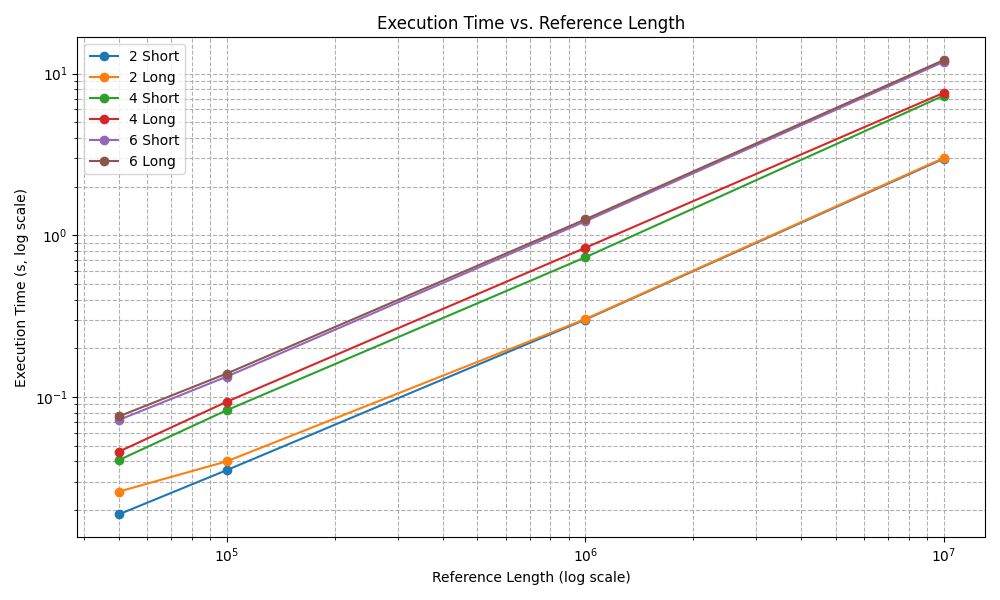
\includegraphics[width=350px]{linearref.png}

  \caption{Execution time as a function of reference length for 2, 4, and 6 inversions, comparing short and long inversions. The plot uses a logarithmic scale on both axes, highlighting the linear relationship between the reference length and execution time, that is consistent with the algorithm's time complexity.}
  \label{fig:refgraph}
\end{figure}

Additionally, the results show that execution times increase almost linearly with the number of inversions \( n \). For instance, at \( r \) = 100000, the time for 2 short inversions was 0.0353 \( s \), while for 6 short inversions, it was 0.1336 \( s \): roughly a 3.7x increase for 3 times the number of inversions.\\
Also evident is a slight but consistent increase in execution time when dealing with longer inversions. For example, at \( r \) = 10000000, the time for 2 short inversions was 0.3009 \( s \), while for 2 long inversions and the same reference length, it was 0.3029 \( s \). The impact of inversion length \( m \) is less pronounced than the impact of \( r \) or \( n \), but still measurable. \\
As \( r \) increases, the difference in execution times between short and long inversions diminishes in relative terms. In fact, at \( r \) = 10000000, the execution time for 2 short inversions is 2.9765 \( s \), while for 2 long inversions is 3.0082 \( s \). The difference is minimal compared to the absolute increase caused by the reference length.

\subsection{With inverted duplications}

Inverted duplications are a type of SV in which a segment of DNA is duplicated and the copy is inserted in the reverse orientation relative to the original. These duplications are often found in genomes and can be associated with various genetic disorders and evolutionary processes \cite{hermetz_large_2014}. In an inverted duplication, the duplicated sequence is typically contiguous with the original, but flipped in orientation, leading to an inverted repeat structure, as summarized in Figure \ref{fig:invd}.

\begin{figure}[h]

  \centering
    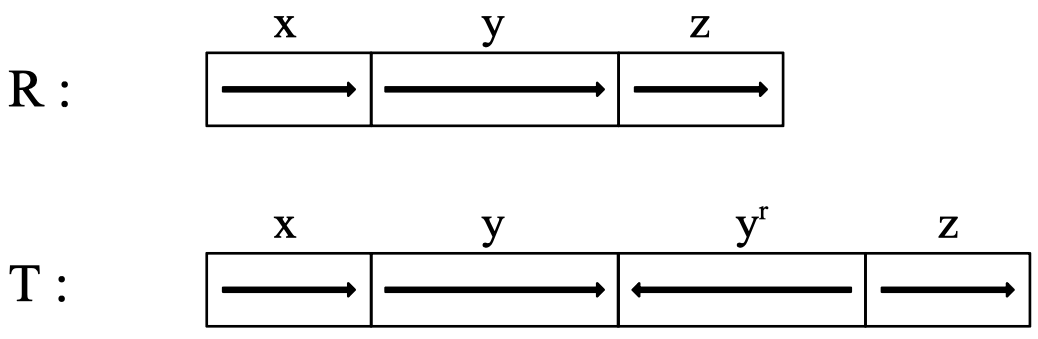
\includegraphics[width=300px]{invd.png}

  \caption{Reference sequence \( R \) and target sequence \( T \) that has undergone an inverted duplication event. In the reference, the sequence consists of three segments, \( x \), \( y \) and \( z \), all oriented in the same direction. However, in the target, the segment \( y \) is duplicated and inserted in the reverse orientation, indicated as \( y^r \).}
  \label{fig:invd}
\end{figure}

In order to generate samples that contain inverted duplications, another \texttt{Python} script was built, \texttt{input\_duplications.py}. It allows setting the reference length, target length, and the start and end indexes of the segment that will be inverted and inserted directly afterward. \\
The experimentation shows that the algorithm can also detect inversions in these situations, since sample-specific strings are detected at the beginning and end of the inverted segment in the target. This segment, when reversed, matches a segment in the reference (see Figure \ref{fig:invd} where, if \( y^r \) is reverted, \( y \) is obtained, which is present in the reference). The next step was to determine the breakpoints, just like in the case without inverted duplications.